\documentclass[tikz]{scrartcl}
\usepackage{tikz}
\newcommand{\<}{\textless}
\renewcommand{\>}{\textgreater}
\usetikzlibrary{calc,positioning, shapes, petri, automata,spy}
\tikzset{
    transV/.style={transition, fill=black,font=\footnotesize, minimum height = 12mm, minimum width = 1.5mm,inner sep = 0mm},
    transH/.style={transition, fill=black,font=\footnotesize, minimum width = 12mm, minimum height = 1.5mm,inner sep = 0mm},
    node distance=1.5
}
\usepackage{amsmath,amssymb,amsthm,mathrsfs,amsfonts}

\usepackage{csquotes}
\usepackage{booktabs}

\usepackage{graphicx}
\graphicspath{ {../img/} }
\usepackage{pgfplots}
    \pgfplotsset{
        table/search path={../performance/measurements},
    }

\newcommand{\LSset}[2]{\scriptsize $\begin{aligned}&\{#1\}_L\\&\{#2\}_S\end{aligned}$}



\begin{document}
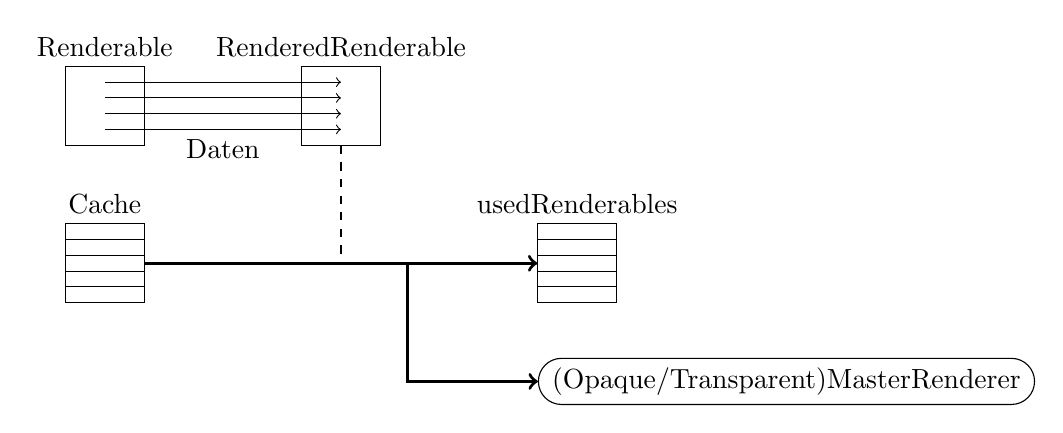
\begin{tikzpicture}
	\usetikzlibrary{calc}
	\node[draw, minimum size = 1cm, label ={RenderedRenderable}] at (0,2) (rr) {};
	\node[draw, minimum size = 1cm, label ={Renderable}] at (-3,2) (r) {};
	\node[draw, minimum size = 1cm, label ={Cache}] at (-3,0) (c) {};
	\node[draw, minimum size = 1cm, label ={usedRenderables}]  at (3,0) (u) {};
	\draw[->, very thick] (c) -- coordinate[pos=.67] (start)  (u);
	\draw[dashed] (rr) -- (0,0);
	\foreach \i in {-.1,.1,.3}{
	\draw[->] ($(r.center)+(0,\i)$) -- ($(rr.center)+(0,\i)$);
	}
	\draw[->] ($(r.center)+(0,-.3)$) -- node[below] {Daten} ($(rr.center)+(0,-.3)$);
	\node[draw,rounded rectangle,anchor=west]  at (2.5,-1.5) (omr) {(Opaque/Transparent)MasterRenderer};
	\draw[->, very thick] (start) |- (omr.west);
	\foreach \i in {-.3,-.1,.1,.3}{
		\draw ($(c.center)+(-.5,\i)$) -- ($(c.center)+(.5,\i)$);
		\draw ($(u.center)+(-.5,\i)$) -- ($(u.center)+(.5,\i)$);
		}
	\end{tikzpicture}
\end{document}